\documentclass[a4paper,11pt]{article}

\usepackage[a4paper,margin=2.3cm]{geometry}
\usepackage{graphicx}
\usepackage[section]{placeins}
\usepackage{cleveref}
\usepackage{listings}
\lstset{
  language=bash,
  basicstyle=\ttfamily
}

\title{Allocation Profiling}
\author{Ruairidh MacGregor}
\date{}

\begin{document}

\maketitle

\section{Info on What Figures Mean}

The figures in this document (so far) are as follows:

\begin{description}
\item \textbf{Access Matrix}: counts the number of accesses made by a thread located on region $i$ accessing memory on region $j$. Note: only pinned threads will give this level of detail, e.g. we know the region where the access is coming from. Unpinned threads are just tracked as unpinned and just shows accesses to a particular region. Accesses made by unpinned threads will be totally random as there location will be determined by the thread scheduler and hence a strong chance of not being overtly consistent between runs. Note: in the current implementation of NUMAPROF, cache hits also appears as memory accesses in the same region, so these aren't solely main memory accesses in the local sense.
\item \textbf{Allocation Matrix}: similar to the \textbf{access matrix}, however, counts allocations. Same rules apply to pinned \& unpinned threads.
\item \textbf{Distance statistics}: a bar chart showing the number of accesses made in the program to a region from a particular distance to the one the thread making the access resides on. \Cref{fig:distance} puts this into a more concrete sense and shows these distances on Togian.
\end{description}

\begin{figure}[!htb]
    \centering
    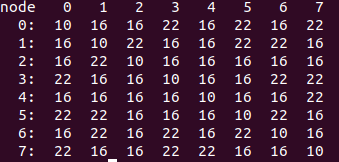
\includegraphics[width=\linewidth]{TechMemo/results/misc/distances.png}
    \caption{Distances between regions on Togian. The distances specified are relative distances, but give an indication of the increased factor of accessing remote regions. Across the diagonal (which corresponds to local accesses) is shown to be 10 which is relative to some baseline access time (I don't know what the baseline is). Accessing remote regions from some region can be either 16 or 22 and I have a strong feeling this is to do with the hardware layout (e.g. something I know absolutely nothing about :)) }
    \label{fig:distance}
\end{figure}

\section{Allocation Metrics}

All results in this document are using GHC 8.4.3 with the --numa flag switched on and using all 64 cores of the 8-region Linux server Togian.

\subsection{Blackscholes}

Commands to reproduce:
\begin{lstlisting}
make clean
make boot EXTRA_HC_OPTS="-threaded"
make EXTRA_HC_OPTS="-threaded"
numaprof ./blackscholes 1000 100000000 +RTS -N --numa -RTS
\end{lstlisting}

\begin{figure}[!htb]
    \centering
    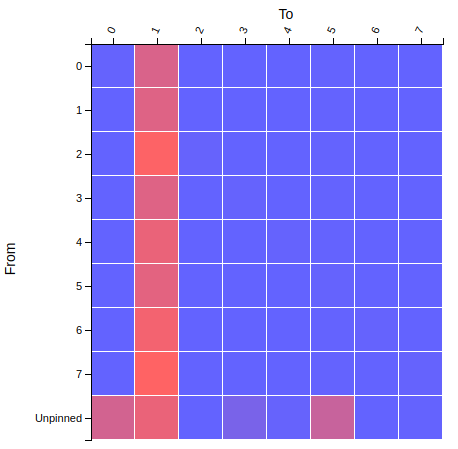
\includegraphics[width=0.5\linewidth]{TechMemo/results/blackscholes/blackscholes_access.png}
    \caption{Access Matrix for blackscholes. Results show  a fairly uniform amount of accesses per region, as indicated by the colour blue being the same across most regions. However, region 1 appears to have a significantly higher amount of accesses compared to the rest. As such, most of these accesses are indeed remote (as it is only region 1 that can perform a local access iin region 1)}
    \label{fig:bscholes_access_matrix}
\end{figure}

\begin{figure}[!htb]
    \centering
    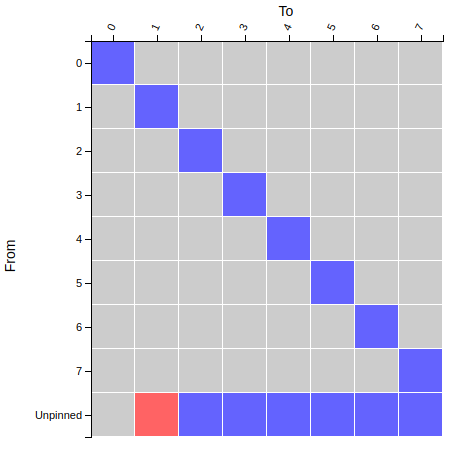
\includegraphics[width=0.5\linewidth]{TechMemo/results/blackscholes/allocation_matrix.png}
    \caption{Allocation Matrix for blackscholes. Following on from the discussion in \Cref{fig:bscholes_access_matrix}, region 1 appears to also have a significant number of allocations compared to elsewhere and is done so by unpinned threads, i.e. not worker threads that are performing the graph reduction as those are pinned. Thus meaning a significant amount of memory allocated by the program is situated in a particular region and hence can be concluded that there is load imbalance issues for this particular application.
    }
    \label{fig:bscholes_alloc_matrix}
\end{figure}

\begin{figure}[!htb]
    \centering
    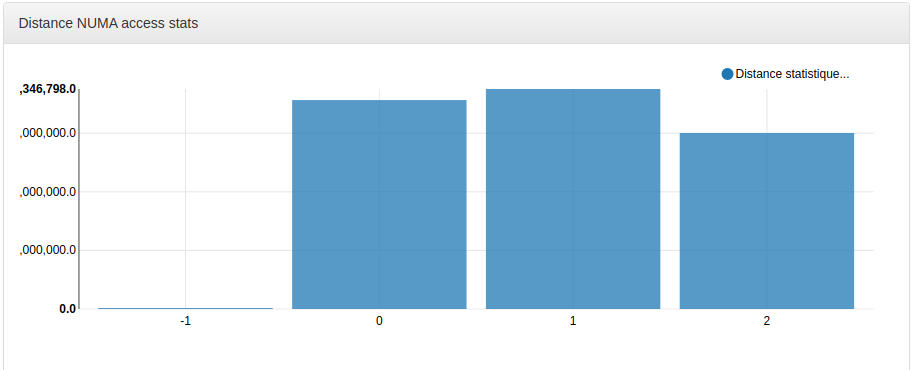
\includegraphics[width=\linewidth]{TechMemo/results/blackscholes/blackscholes_distance.png}
    \caption{Distance statistics for blackscholes. The types of accesses are fairly similar across all 3 possible distances. Showing mostly accesses at distance 1, e.g relative to a factor of 16 (\Cref{fig:distance}). Observing the accessing matrix in \Cref{fig:bscholes_access_matrix}, the accesses do largely appear uniform across most regions, with the exception being region 1.}
    \label{fig:blackscholes_distance}
\end{figure}


\subsection{parfib}

Commands to reproduce run with:
\begin{lstlisting}
make clean
make boot EXTRA_HC_OPTS="-threaded"
make EXTRA_HC_OPTS="-threaded"
numaprof ./parfib 88 7 +RTS -N --numa -RTS
\end{lstlisting}

\begin{figure}[!htb]
    \centering
    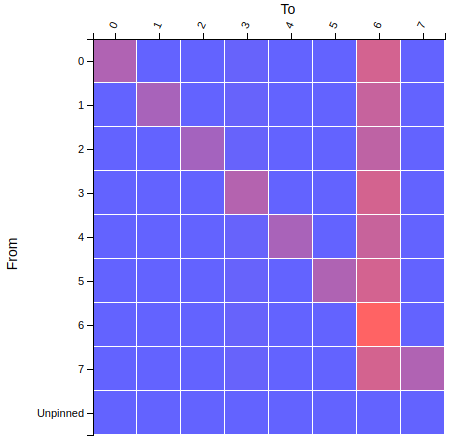
\includegraphics[width=0.5\linewidth]{TechMemo/results/parfib/parfib_access.png}
    \caption{Access Matrix for parfib. Results show strong locality awareness, indicated by the stronger purple/red like colour across the diagonal, as these correspond to local accesses. However, just as with blackscholes there is an imbalance, with this case being in region 6.}
    \label{fig:parfib_access_matrix}
\end{figure}

\begin{figure}[!htb]
    \centering
    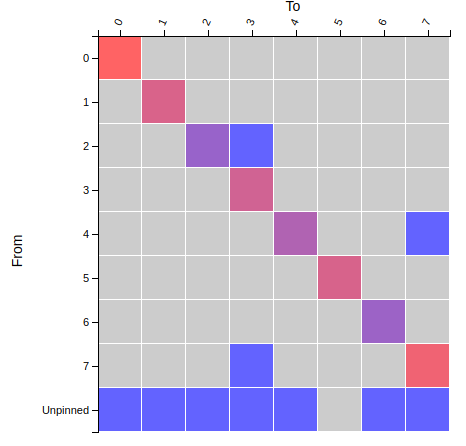
\includegraphics[width=0.5\linewidth]{TechMemo/results/parfib/parfib_alloc.png}
    \caption{Allocation Matrix for parfib. Results show a significantly higher number of allocations done by pinned threads, e.g. the worker threads performing graph reduction. Results do indeed show strong locality awareness, which correlates well with the access matrix in \Cref{fig:parfib_access_matrix} and minimal amounts of allocations done in separate regions. Observing the allocations done in region 6, which appears to have a significantly high amount of accesses too done by all other regions, doesn't really show a significant amount. Region 0 and 7 appear to be the highest. Reasons for this mismatch could be down the garbage collection moving data originally allocated in these regions to region 7. Or perhaps, the allocations made in this region were large objects that were used across regions fairly frequent.}
    \label{fig:parfib_alloc_matrix}
\end{figure}

\begin{figure}[!htb]
    \centering
    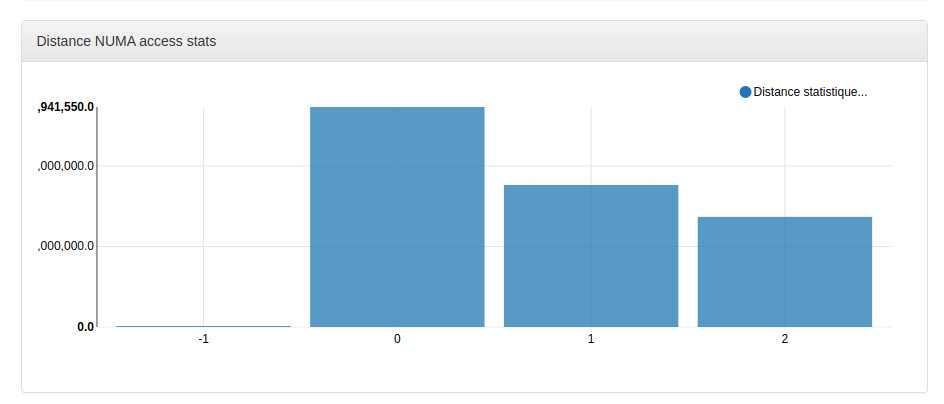
\includegraphics[width=\linewidth]{TechMemo/results/parfib/parfib_distance.png}
    \caption{Distance statistics for parfib. Results show that most accesses do in fact appear to be local overall, indicated by the bar with distance 0 (10) being the highest, with distances 1 (16) being second largest and 2(22) being the smallest. So this does show a sound adotion of NUMA distance accesses. However, I am not overly sure the GHC RTS takes this into account, this may just be luck. }
    \label{fig:parfib_distance}
\end{figure}

\subsection{matmult}

Commands to reproduce:
\begin{lstlisting}
make clean
make boot EXTRA_HC_OPTS="-threaded"
make EXTRA_HC_OPTS="-threaded"
numaprof ./matmult +RTS -N --numa -RTS
\end{lstlisting}

\begin{figure}[!htb]
    \centering
    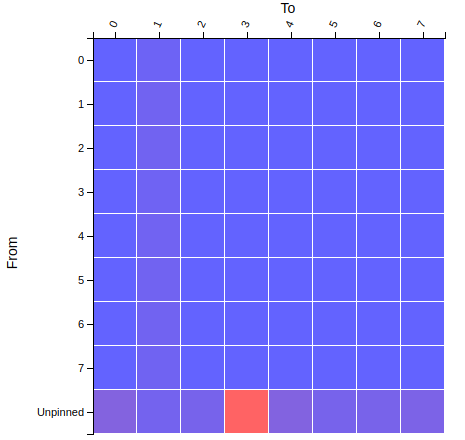
\includegraphics[width=0.5\linewidth]{TechMemo/results/matmult/matmult_accessMatrix.png}
    \caption{Access Matrix for matmult. Results show fairly similar accesses across regions, with the exception being region 1 that has a stronger purple-like colour (indicating higher accesses)}
    \label{fig:matmult_access_matrix}
\end{figure}

\begin{figure}[!htb]
    \centering
    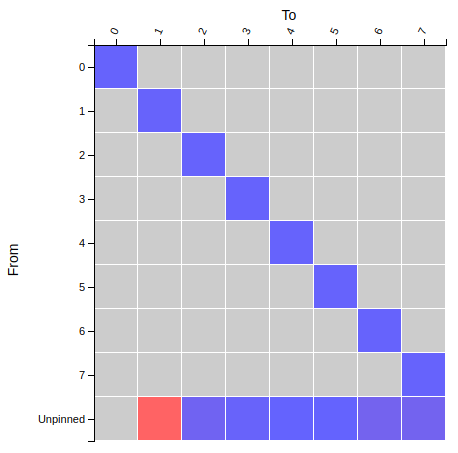
\includegraphics[width=0.5\linewidth]{TechMemo/results/matmult/matrix_mult_allocMatrix.png}
    \caption{Allocation Matrix for matmult}
    \label{fig:matmult_alloc_matrix}
\end{figure}

\begin{figure}[!htb]
    \centering
    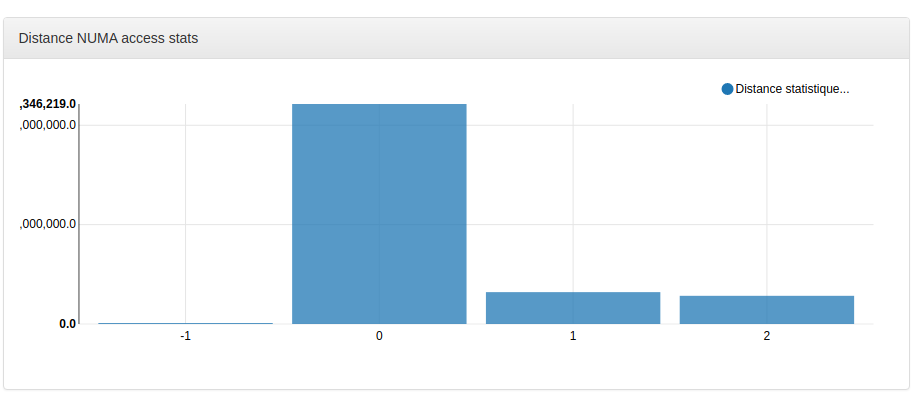
\includegraphics[width=\linewidth]{TechMemo/results/matmult/matmult_distance.png}
    \caption{Distance statistics for matmult}
    \label{fig:matmult_distance}
\end{figure}

\subsection{quicksort}

Commands to reproduce:
\begin{lstlisting}
# Note: the quicksort directory did not have a makefile
ghc -threaded QuickSortD.hs -o QuickSortD
numaprof ./QuickSortD +RTS -N --numa -RTS
\end{lstlisting}

\begin{figure}[!htb]
    \centering
    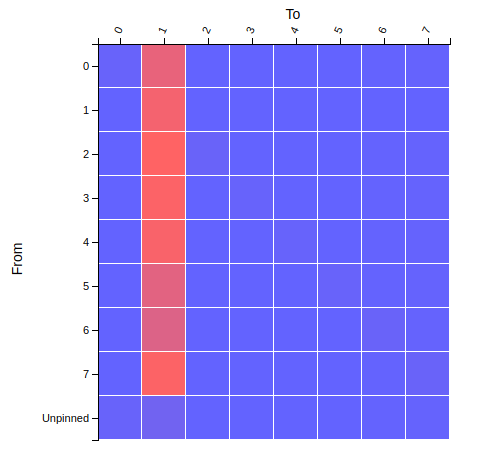
\includegraphics[width=0.5\linewidth]{TechMemo/results/quicksort/access_matrix.png}
    \caption{Access Matrix for quicksort.}
    \label{fig:quicksort_access_matrix}
\end{figure}

\begin{figure}[!htb]
    \centering
    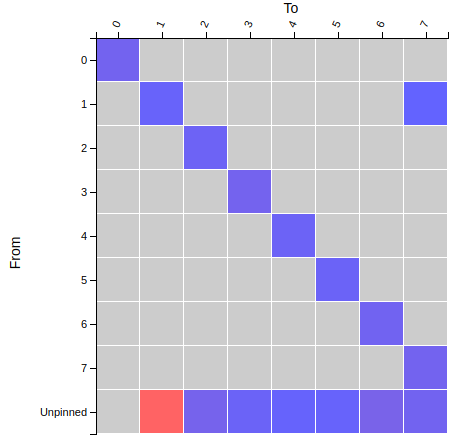
\includegraphics[width=0.5\linewidth]{TechMemo/results/quicksort/alloc_quicksort_.png}
    \caption{Allocation Matrix for quicksort.}
    \label{fig:quicksort_alloc_matrix}
\end{figure}

\begin{figure}[!htb]
    \centering
    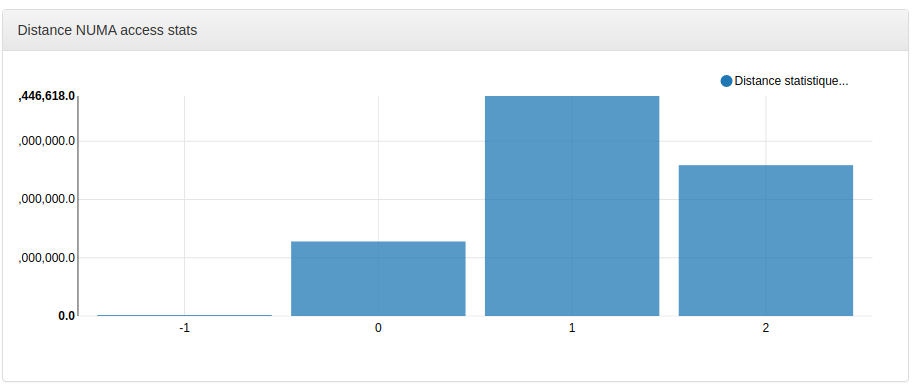
\includegraphics[width=\linewidth]{TechMemo/results/quicksort/quicksort_distance.png}
    \caption{Distance statistics for quicksort.}
    \label{fig:quicksort_distance}
\end{figure}

\subsection{sumeuler}

Commands to reproduce:
\begin{lstlisting}
make clean
make boot EXTRA_HC_OPTS="-threaded"
make EXTRA_HC_OPTS="-threaded"
numaprof ./sumeuler 38 300000 400 +RTS -N  --numa -RTS 
\end{lstlisting}

\begin{figure}[!htb]
    \centering
    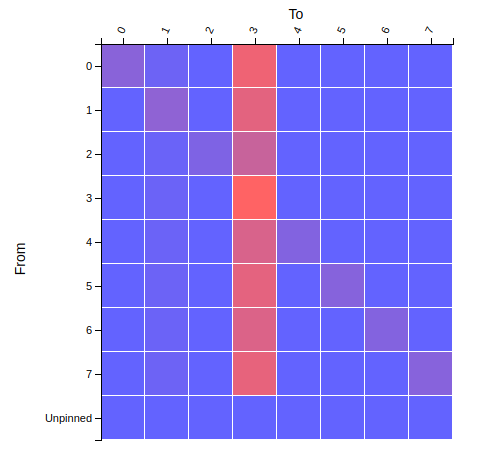
\includegraphics[width=0.5\linewidth]{TechMemo/results/sumeuler/sumeukler_access.png}
    \caption{Access Matrix for sumeuler.}
    \label{fig:sumeuler_access_matrix}
\end{figure}

\begin{figure}[!htb]
    \centering
    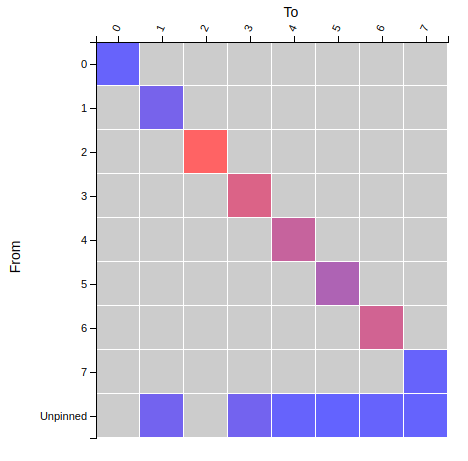
\includegraphics[width=0.5\linewidth]{TechMemo/results/sumeuler/alloc_sumeuler.png}
    \caption{Allocation Matrix for sumeuler.}
    \label{fig:sumeuler_alloc_matrix}
\end{figure}

\begin{figure}[!htb]
    \centering
    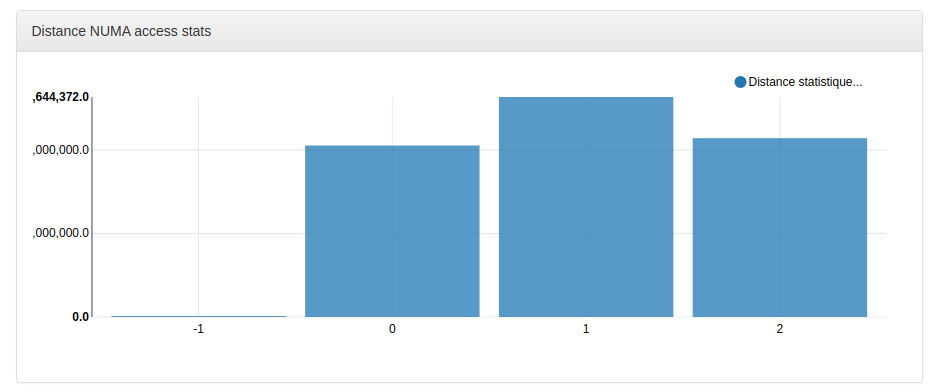
\includegraphics[width=\linewidth]{TechMemo/results/sumeuler/distance_sumeuler.png}
    \caption{Distance statistics for sumeuler}
    \label{fig:sumeuler_distance}
\end{figure}

\subsection{prsa}

Commands to reproduce:
\begin{lstlisting}
make clean
make boot EXTRA_HC_OPTS="-threaded"
make EXTRA_HC_OPTS="-threaded"
numaprof ./prsa 432846381 +RTS -N --numa -RTS
\end{lstlisting}

\begin{figure}[!htb]
    \centering
    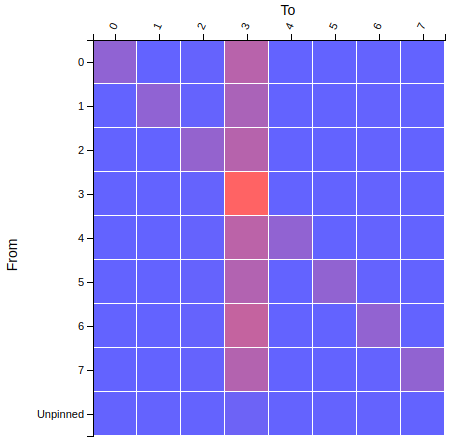
\includegraphics[width=0.5\linewidth]{TechMemo/results/prsa/prsa_access.png}
    \caption{Access Matrix for prsa.}
    \label{fig:prsa_access_matrix}
\end{figure}

\begin{figure}[!htb]
    \centering
    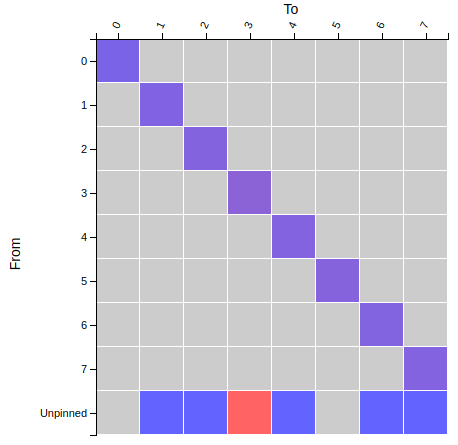
\includegraphics[width=0.5\linewidth]{TechMemo/results/prsa/prsa_allioc.png}
    \caption{Allocation Matrix for prsa.}
    \label{fig:prsa_alloc_matrix}
\end{figure}

\begin{figure}[!htb]
    \centering
    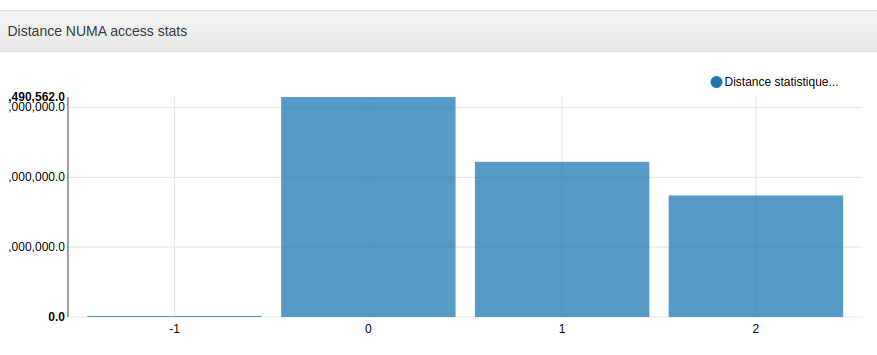
\includegraphics[width=\linewidth]{TechMemo/results/prsa/prsa_distance.png}
    \caption{Distance statistics for prsa.}
    \label{fig:prsa_distance}
\end{figure}

\subsection{cfd}

Commands to reproduce:
\begin{lstlisting}
make clean
make boot EXTRA_HC_OPTS="-threaded"
make EXTRA_HC_OPTS="-threaded"
./cfd +RTS -N --numa -RTS
\end{lstlisting}

\begin{figure}[!htb]
    \centering
    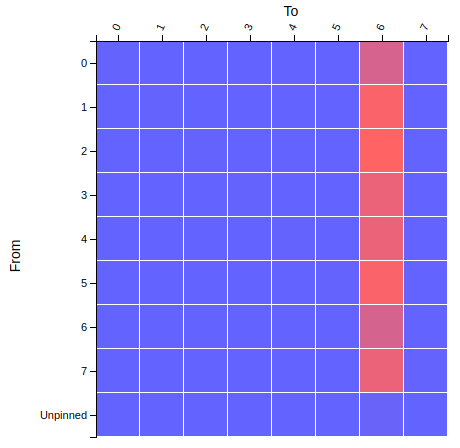
\includegraphics[width=0.5\linewidth]{TechMemo/results/cfd/cfd_access.png}
    \caption{Access Matrix for cfd.}
    \label{fig:cd_access_matrix}
\end{figure}

\begin{figure}[!htb]
    \centering
    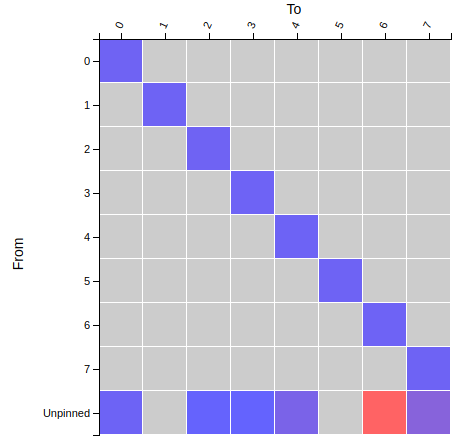
\includegraphics[width=0.5\linewidth]{TechMemo/results/cfd/alloc_Cfd.png}
    \caption{Allocation Matrix for cfd.}
    \label{fig:cfd_alloc_matrix}
\end{figure}

\begin{figure}[!htb]
    \centering
    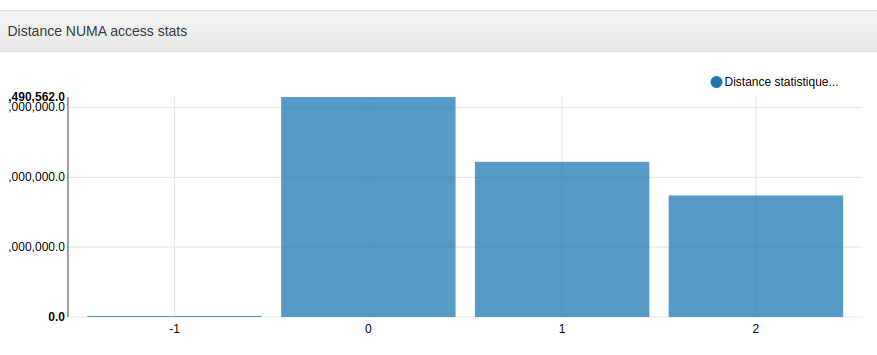
\includegraphics[width=\linewidth]{TechMemo/results/prsa/prsa_distance.png}
    \caption{Distance statistics for cfd.}
    \label{fig:cfd_distance}
\end{figure}

\subsection{General Comments}

Observing all the access matrices, there appears to be a common pattern of an overly accessed region compared to others, with the exception of matmult in \Cref{fig:matmult_access_matrix}, which appears to be fairly uniform across all regions. It is unclear whether this is initially due to load balancing policies implemented, e.g. some regions can become overpopulated and use remote regions, however, the policy could be failing and choosing to do move data to the region that has significantly higher accesses. Overall, this type of profiling information could be very beneficial inside the runtime system itself to allow the system to have a coherent view of what types of accesses are being made and if there is overly accessed regions, so the system could adapt if this starts becoming a bottleneck (although, good luck implementing it to (A) keep track of necessary objects and (B) not introduce too much overhead). Another general observation with regards to accesses is that there is never really a clear sense of locality from the matrices. In particular, the region along the diagonal appears to be fairly similar in colour to all other regions, e.g. blue, with the exception being in \Cref{fig:parfib_access_matrix}, that shows a more inherent sense of locality across the diagonal, however, again with a region that appears to have a significantly high number of accesses.

On the flip-side, in almost all cases with the exception of \cref{fig:parfib_alloc_matrix}, the initial allocations made by GHC worker threads appear to be always allocating locally. Indicated by the only shade of colour appearing on the diagonal for pinned threads. Another observation in the cases of \Cref{fig:sumeuler_alloc_matrix} and \Cref{fig:parfib_alloc_matrix}, there appears to be relatively imbalance between allocations made by threads in particular regions. More specifically, some regions appear to have much higher allocations than others, indicated by the inherently strong red/purple colours.

The distance statistics appear to show good locality in \Cref{fig:parfib_distance} and \Cref{fig:matmult_distance} with the highest being bar being distance 0 (e.g. 10 in \Cref{fig:distance}). The rest appear to show a fairly similar amount of accesses in each, indicated by the height of each bar being fairly similar, however, distance 1 (16) appears to be the most favourable.

%\section{De-allocation Metrics}

\end{document}